\documentclass[11pt]{standalone}
\usepackage{amssymb}
\usepackage{amsmath}
\usepackage[no-math]{fontspec}
\usepackage{unicode-math}
\usepackage{libertinus}
\usepackage{pgf,xcolor}
\usepackage{tikz}
\usetikzlibrary{arrows.meta, backgrounds}
\usepackage{pgfplots}
\pgfplotsset{compat=newest}

\definecolor{my_darkgray}{HTML}{484949}
\definecolor{my_lightgray}{HTML}{F3F4F4}
\definecolor{my_darkblue}{HTML}{005A94}
\definecolor{my_lightblue}{HTML}{CCDEE9}
\definecolor{my_yellow}{HTML}{FFEC7F}
\definecolor{my_red}{HTML}{E60000}
\definecolor{my_orange}{HTML}{E87846}

\begin{document}
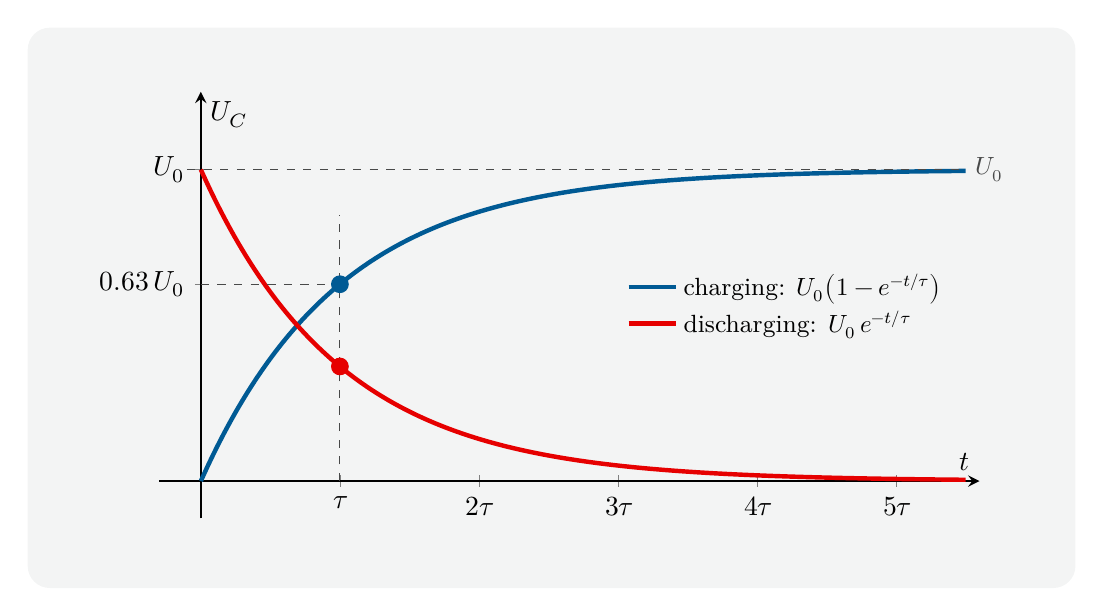
\begin{tikzpicture}[
    show background rectangle,
    background rectangle/.style={fill=my_lightgray, rounded corners=8pt},
    inner frame sep=0.8cm
]
\begin{axis}[
    axis lines=center,
    xlabel={$t$},
    ylabel={$U_C$},
    height=7cm, width=12cm,
    xmin=-0.3, xmax=5.6,
    ymin=-0.12, ymax=1.25,
    xtick={1, 2, 3, 4, 5},
    xticklabels={$\tau$, $2\tau$, $3\tau$, $4\tau$, $5\tau$},
    ytick={0, 0.632, 1},
    yticklabels={$0$, $0.63\,U_0$, $U_0$},
    axis line style={thick},
    grid=none,
    clip=false,
    legend style={
        font=\small,
        at={(0.97, 0.50)},
        anchor=east,
        draw=none,
        fill=my_lightgray,
    },
    legend cell align=left,
]

% Charging curve: U_C(t) = U_0(1 - e^{-t/tau}), normalized U_0=1, tau=1
\addplot[draw=my_darkblue, samples=300, ultra thick, domain=0:5.5]
    {1 - exp(-x)};
\addlegendentry{charging: $U_0\!\left(1-e^{-t/\tau}\right)$}

% Discharging curve: U_C(t) = U_0 * e^{-t/tau}
\addplot[draw=my_red, samples=300, ultra thick, domain=0:5.5]
    {exp(-x)};
\addlegendentry{discharging: $U_0\, e^{-t/\tau}$}

% Asymptote at U_0 = 1
\addplot[draw=my_darkgray, dashed, thin, domain=-0.1:5.5]{1};

% Dashed vertical line at t = tau = 1
\draw[dashed, my_darkgray, thin] (axis cs:1, 0) -- (axis cs:1, 0.854);

% Dashed horizontal line at 0.632 (= 1 - 1/e), connecting both curves
\draw[dashed, my_darkgray, thin]
    (axis cs:0, 0.632) -- (axis cs:1, 0.632);

% Mark the two characteristic points at t = tau
% Charging: (tau, 1-1/e) ~ (1, 0.632)
\addplot[only marks, mark=*, mark size=3pt,
         draw=my_darkblue, fill=my_darkblue]
    coordinates{(1, 0.632)};

% Discharging: (tau, 1/e) ~ (1, 0.368)
\addplot[only marks, mark=*, mark size=3pt,
         draw=my_red, fill=my_red]
    coordinates{(1, 0.368)};

% Label U_0 on right edge of asymptote
\node[right, font=\small, my_darkgray] at (axis cs:5.5, 1.0) {$U_0$};

\end{axis}
\end{tikzpicture}
\end{document}
